\chapter{Entorno de Trabajo}\label{cap:07diseño}

Este capítulo presenta el entorno de trabajo: \ref{sec:07arqTecno} la arquitectura tecnológica y \ref{sec:07entorno} el entorno tecnológico.

\section{Introducción}

La implementación del ecosistema de herramientas OHDSI y ATLAS puede ser una ardúa tarea. En el contexto de desarrollo del Trabajo Fin de Grado junto a las prácticas en empresa en el Hospital Virgen del Rocío, la dificultad de la tarea se ve exponencialmente aumentada debido a los grandes protocolos de seguridad y privacidad de la administración pública. Por ello, se ha seleccionado el despliegue de las herramientas OHDSI a través del subsistema Docker de Broadsea, que presenta una vía sencilla para realizar esta labor. 

Broadsea es un proyecto basado en Docker que permite desplegar todo el entorno de herramientas, configuraciones y dependencias OHDSI de la manera más sencilla hasta el momento. De hecho, la misma organización la presenta, textualmente, como \textit{''la forma más sencilla de instalar (y actualizar) las herramientas OHDSI"} \cite{Broadsea3PDF}. 

\begin{figure}[H]
    \centering
    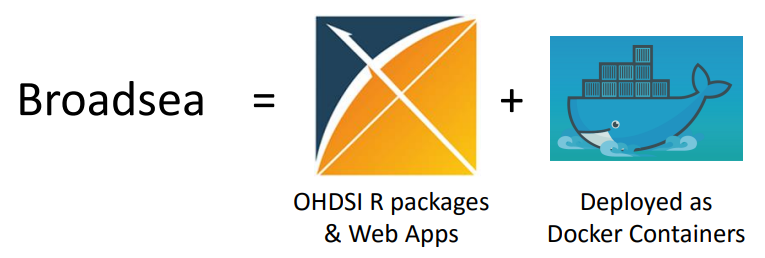
\includegraphics[width=0.70\textwidth]{figures/broadseaEq.png}
    \caption{Esquema sencillo de Broadsea. Extraída de \cite{Broadsea3PPTX}.}
    \label{fig:broadseaEq}
\end{figure}

Aunque comenzó en su primera versión, como un simple contenedor que albergase imágenes de la WebAPI de ATLAS y RStudio \cite{Broadsea3PPTX} ha evolucionado hasta la tercera versión en la que Broadsea alberga la mayoría de herramientas OHDSI, creando un entorno virtual de desarrollo muy completo.

\begin{figure}[H]
    \centering
    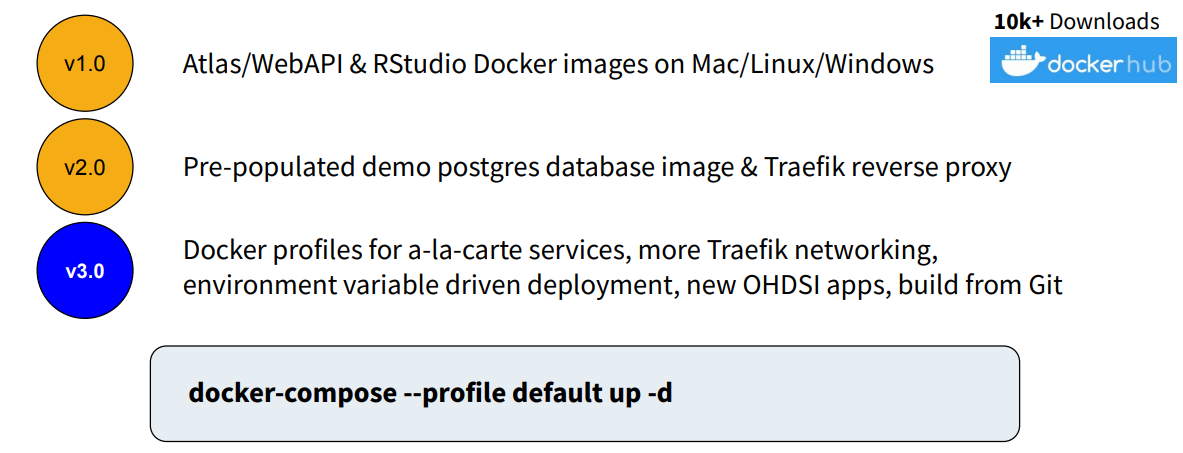
\includegraphics[width=0.90\textwidth]{figures/versionesBroadsea.png}
    \caption{Historial de versiones de Broadsea. Extraída de \cite{Broadsea3PPTX}.}
    \label{fig:versionesBroadsea}
\end{figure}

La tercera versión de Broadsea incluye perfiles docker que facilitan la configuración del servicio, redes internas de conexión, despliegue de variables internas, más aplicaciones OHDSI y la construcción de contenedores desde Git, entre otros. 

A continuación se presenta la arquitectura teórica de Broadsea y el entorno de herramientas tecnológicas necesarias para su correcta implementación.

\section{Arquitectura tecnológica} \label{sec:07arqTecno}

La arquitectura en términos tecnológicos del sistema es compleja, por ello se describe en dos subsecciones: \ref{subsec:07sistema} Arquitectura teórica-generalizada del sistema y \ref{subsec:07Broadsea} Arquitectura específica de Broadsea.

\subsection{Arquitectura del sistema}\label{subsec:07sistema}

El sistema se implementa mediante virtualización con Docker y una arquitectura en tres niveles o \textit{three-tier}, donde se diferencian al cliente, frontend y backend. Esta arquitectura se describirá de forma general utilizando el esquema de la Figura \ref{fig:threetierDocker}, extraído de internet.

\begin{figure}[H]
    \centering
    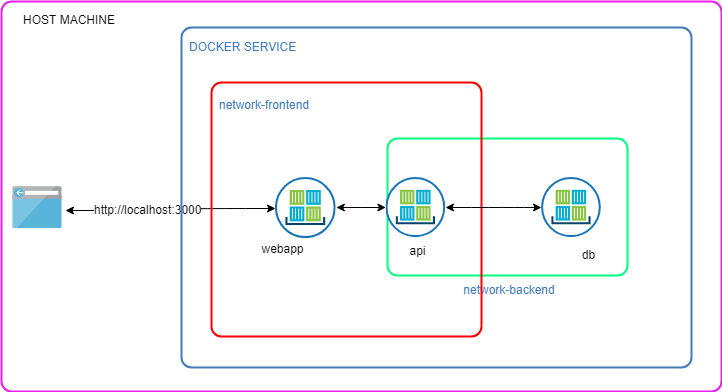
\includegraphics[width=0.80\textwidth]{figures/threetierDocker.png}
    \caption{Esquema de arquitectura \textit{three-tier} en Docker. Extraída de \cite{threetierDocker}.}
    \label{fig:threetierDocker}
\end{figure}

En primer lugar, la virtualización obliga a diferenciar entre una maquina local o anfitriona (\textit{host machine}, en rosa) y una maquina virtual que provee el servicio docker (\textit{docker service}, en azul). 

\begin{enumerate}

    \item \textbf{La máquina local.} La máquina local es la propia máquina del usuario. Se le denomina anfitriona porque aloja en su interior a la máquina virtual. La máquina local cede un servidor y un puerto a la máquina virtual para que el usuario final pueda acceder al sistema a través de la dirección del servidor en que se aloja, típicamente accediendo mediante un navegador web. El acceso mediante el navegador web es lo que se denomina la capa cliente, pues es la interfaz que permite al usuario acceder al sistema. 

    \item \textbf{La máquina virtual.} La máquina virtual es el sistema virtualizado en Docker. Es el sistema que contiene toda la lógica de la aplicación y los datos empaquetado en un multicontenedor Docker, en este caso el multicontenedor es el propio sistema Broadsea. Está compuesto por tres nodos la \textit{webapp}, la \textit{api} y la \textit{db} que conforman las dos capas restantes de la arquitectura: el frontend y el backend.
    
\end{enumerate}

Por tanto, a nivel de aquitectura del sistema en sí, se encuentra la capa cliente (en el \textit{host machine}, en rosa), el frontend (\textit{network-frontend}, en rojo) y el backend (\textit{network-backend}, en verde).

\begin{enumerate}

    \item \textbf{El cliente.} El cliente está alojado en la máquina anfitriona y proporciona el acceso a los servicios virtualizados del sistema a través de la conexión internet con el servidor docker.

     En el caso de Broadsea el navegador deberá ser Google Chrome y la dirección por defecto será http://127.0.0.1:5432.

    \item \textbf{El frontend.} El frontend está alojado en la máquina virtual, es el servicio que guarda la lógica de la aplicación que se muestra al usuario. Se compone de la \textit{webapp}, que contiene la aplicación como tal, y la \textit{api}. que es la red que permite establecer interconexiones entre la aplicación lógica y la base de datos; entre el frontend y el backend.

    En el caso de Broadsea la webapp y la api se combinan en el componente de la WebAPI, que permite el acceso a la aplicación de ATLAS y maneja las conexión con las bases de datos del backend.

    \item \textbf{El backend.} El backend está alojado en la máquina virtual, es el servicio que aloja la base de datos sobre la que se sostiene la aplicación. Se compone de la \textit{api} y la \textit{db}. De igual forma que en el frontend, la api es la red que permite la interconexión entre los componentes del sistema, en este caso con la base de datos, que puede ser una o varias.

    En el caso de Broadsea, las bases de datos deberán estar estandarizadas a OMOP y podrán encontrarse en el propio servidor Docker, como es el caso de Eunomia, o en servidores externos. No obstante, la relación entre cualquier base de datos y ATLAS se realiza a través de la WebAPI.

    
\end{enumerate}

\subsection{Arquitectura de Broadsea} \label{subsec:07Broadsea}

%Presentación del sistema Broadsea. Imagen de Broadsea

A continuación se presenta la aquitectura específica de Broadsea. Broadsea v3.0 es un sistema muy complejo, contenido en un multicontenedor Docker que alberga el ecosistema completo de herramientas OHDSI y sus interconexiones en distintos contenedores. Además, se definen distintos perfiles (\textit{profiles}) para facilitar la instalación de los distintos contenedores. Por ello se le denomina \textit{a-la-carte}. La figura \ref{fig:OHDSIBroadsea3.0} muestra todos los contenedores de Broadsea.

\begin{figure}[H]
    \centering
    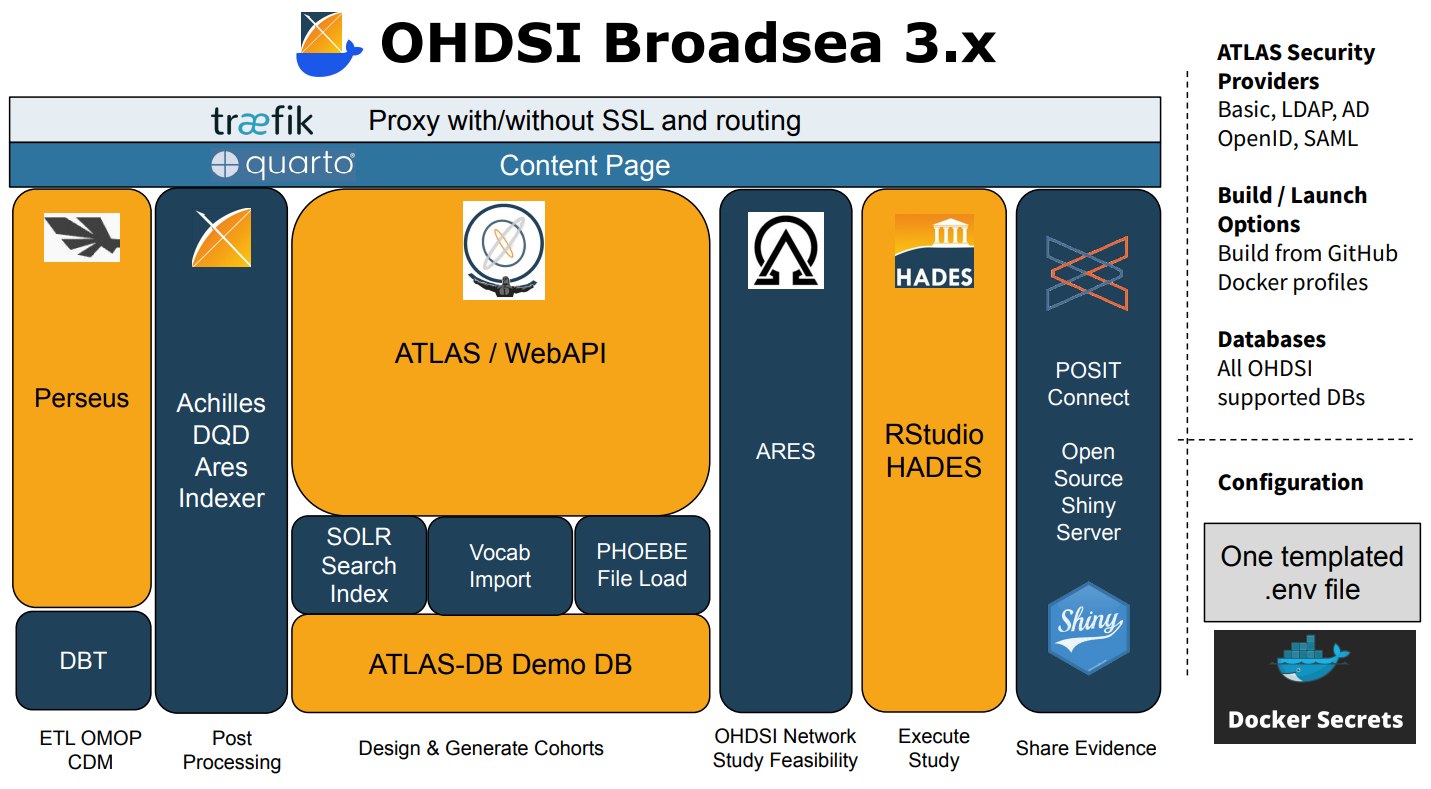
\includegraphics[width=0.90\textwidth]{figures/OHDSIBroadsea3.0.png}
    \caption{Vista general de todos los componentes de Broadsea. Extraída de \cite{Broadsea3PPTX}.}
    \label{fig:OHDSIBroadsea3.0}
\end{figure}

El despliegue por defecto de Broadsea genera en el frontend una interfaz de usuario con acceso a tres aplicaciones: ATLAS, HADES y ARES. Para acceder a esta interfaz de usuario basta con buscar en el navegador el servidor y puerto donde se aloja broadsea, que tipicamente será la maquina local y el puerto 5354, correspondiente a Postgre.

\begin{enumerate}

    \item \textbf{ATLAS}. ATLAS Broadsea despliega todas las funcionalidades de la herramienta de forma local. ATLAS se sostiene sobre la WebAPI y cuenta con la base de datos de Eunomia.
    
    \begin{enumerate}
        \item \textbf{WebAPI}. La WebAPI se despliega como un contenedor docker y como un volumen de datos. Además, también se construirá un esquema en la base de datos del servidor Postgre que aloja al contenedor, denominado \code{webapi}. A través de la modificación de este esquema se podrán agregar o eliminar las diferentes fuentes de datos a la herramienta.
        \item \textbf{BD}. Para facilitar el correcto funcionamiento de ATLAS se implementa una base de datos demo que es Eunomia. Esta base de datos cuenta con un pequeño registro de datos normalizados a OMOP y también crea varios esquemas en la base de datos del servidor Postgre que permiten su configuración, o la realización de consultas directamente desde el administrador de la base de datos.
    \end{enumerate}

    \item \textbf{HADES}. HADES Broadsea despliega todas las funcionalidades de la herramienta de forma local. Se sostiene sobre una virtualización del IDE de RStudio que tiene preinstalada y preconfiguradas todas las librerías de la Librería de Métodos. Su uso no es relevante en el TFG.
   
    \item \textbf{ARES}. ARES Broadasa despliega todas las funcionalidades de la herramienta de forma local. Su uso tampoco es relevante en el TFG.

\end{enumerate}



\section{Entorno tecnológico} \label{sec:07entorno}

El entorno tecnológico que envuelve al sistema está compuesto por cuatro herramientas fundamentales: Docker, PostgreSQL, Google Chrome y Github.


\subsection{Google Chrome}

Google Chrome es el navegador web de Google que permite el acceso a internet y la búsqueda en la web a través de una interfaz amigable e intuitiva \cite{GoogleChrome}. 

El uso de Chrome para el acceso a Broadsea es muy recomendado por los propios desarrolladores, por lo que es una herramienta de especial relevancia.

\subsection{Docker}

Docker es una plataforma abierta para desarrollar, enviar y ejecutar aplicaciones. Docker le permite separar sus aplicaciones de su infraestructura para que pueda entregar software rápidamente. Con Docker, puede administrar su infraestructura de la misma manera que administra sus aplicaciones \cite{DockerWebsite}.

De esta forma, Docker permite empaquetar y ejecutar aplicaciones en contenedores, entornos poco aislados pero seguros. Esto posibilita la ejecución de múltiples contenedores simultáneamente en un mismo host, sin depender de lo instalado en él. Los contenedores son ligeros y contienen todo lo necesario para la aplicación, facilitando su compartición y asegurando consistencia entre usuarios. 

El uso de Docker en el desarrollo del TFG es evidente, es la herramienta que despliega Broadsea y, por consiguiente, ATLAS (véase \ref{sec:07Broadsea}). El proceso concreto de instalación, despliegue y configuración de Docker así como la explicación detallada de su estructura y archivos más importantes se presenta en el anexo \ref{anexo:manual}.

\subsection{PostgreSQL}

PostgreSQL es un potente sistema de base de datos relacional de objetos de código abierto que utiliza y amplía el lenguaje SQL combinado con muchas funciones que almacenan y escalan de forma segura las cargas de trabajo de datos más complicadas \cite{PostgreWebsite}.

El uso de postgre es fundamental para la implementación correcta de Broadsea, puesto que la WebAPI se implementa sobre un sistema PostgreSQL. Las bases de datos externas que se interactúan con la WebAPI pueden estar en otros lenguajes relacionales, pero el sistema de Broadsea intrínsicamente solo se sostiene sobre Postgre.

De nuevo, el proceso concreto de instalación, despliegue y configuración de la base de datos Postgre así como la explicación detallada de su estructura y archivos más importantes se presenta en el anexo \ref{anexo:manual}.

\subsection{Github}

GitHub es una plataforma para desarrolladores que les permite crear, almacenar, gestionar y compartir su código. Utiliza el software Git, proporcionando control de versiones distribuido, además de control de acceso, seguimiento de errores, solicitudes de funciones de software, gestión de tareas, integración continua y wikis para cada proyecto \cite{GithubWikipedia}.

El uso de Github es muy recomendado debido a que la mayor parte de la información sobre OHDSI y sus herramientas se encuentran en internet disponibles en repositorios de Github (véase \ref{sec:05OHDSI}). 

Además, siguiendo esta iniciativa de OHSI, para desarrollar este Trabajo Fin de Grado se ha creado un repositorio de Github específico \cite{vallealonsodc} que contiene toda la documentación relevante a su desarrollo (archivos latex, pdf...) y archivos de variables de entorno o scripts utilizados durante la configuración del entorno del sistema o la realización del análisis de datos.   

\section{Conclusiones}

En este capítulo se concluye que la arquitectura tecnológica del sistema es bastante compleja (véase \ref{sec:07arqTecno}), puesto que involucra una virtualización del ecosistema OHDSI a través de Docker, denominado Broadsea. No obstante, la implementación del sistema en Docker facilita bastante la tarea de configurar el ecosistema completo, gracias al empaquetamiento de las funcionalidades en contenedores accesibles \textit{a-la-carte}. Por último, es importante conocer el entorno tecnológico fundamental para desplegar correctamente el sistema, compuesto por Chrome, Docker, PostgreSQL y Github (véase \ref{sec:07entorno}).